\documentclass{article}
\usepackage{graphicx}
\usepackage{float}
\usepackage{titlesec}
\usepackage{datetime}
\usepackage{geometry}
\usepackage{minted}
\usepackage{placeins}
\usepackage{caption}
\usepackage[document]{ragged2e}
\usepackage[hidelinks]{hyperref}
\usepackage{enumitem}
\geometry{
 a4paper,
 left=25mm,
 top=25mm,
 }
\captionsetup{hypcap=false} 
\newdateformat{daymonthyear}{\THEDAY .\THEMONTH .\THEYEAR}
\title{
  \centering
  
\includegraphics[width=\textwidth]{images/logo_PWr_kolor_poziom.png}\\
  \fontsize{28pt}{30pt}\selectfont Sprawozdanie 4\\
  }
\author{Krzysztof Zalewa}
\date{\daymonthyear\today}
\renewcommand*\contentsname{Spis treści}
\renewcommand{\figurename}{Rysunek}
\renewcommand{\listingscaption}{Skrypt}
\begin{document}
    \maketitle
    \pagebreak
    \tableofcontents
    \FloatBarrier
    \raggedright
    \section{Cel skryptu}
        Celem zadania laboratoryjnego było nauczenie się obsługi komendy nc. 
        Do tego celu stworzono 3 proste skrypty:
        \begin{enumerate}
            \item Skrypt łączący się z localhostem na porcie 12345. 
            Jest najproszy i najkrótszy z trzech.
            \item Skrypt łączący się z wybranym IP na porcie 12345.
            Niewiele dłuższy od skryptu 1. 
            Potrzeba jawnie zapisać IP z którym się łączymy.
            \item Skrypt to prosty "serwer". 
            Po otzymaniu połączenia zwiększany jest licznik i do klienta wysyłane jest HTTP OK (Dla przeglądarki). 
            Następnie wysyłany jest prosty plik html zawierający licznik i datę i godzinę.
        \end{enumerate} 
    \section{Opis skryptu}
        \begin{frame}
            \scriptsize
            \inputminted[
                style={vs},
                breaklines,
                breakanywhere, 
                linenos, 
                tabsize=4 
            ]{bash}{./lab4_1.sh}
            \vspace{1em}
            \captionof{listing}{Połączenie z localhostem na porcie 12345}
            \label{lst:script_1}
        \end{frame}
      
        \begin{frame}
            \scriptsize
            \inputminted[
                style={vs},
                breaklines,
                breakanywhere, 
                linenos, 
                tabsize=4 
            ]{bash}{./lab4_2.sh}
            \vspace{1em}
            \captionof{listing}{Połączenie z wybranym Ip na porcie 12345}
            \label{lst:script_2}
        \end{frame}

        \begin{frame}
            \scriptsize
            \inputminted[
                style={vs},
                breaklines,
                breakanywhere, 
                linenos, 
                tabsize=4 
            ]{bash}{./lab4_3.sh}
            \vspace{1em}
            \captionof{listing}{Prosty "serwer" odpowiadający na zapytania plikem html z zwiększającym się licznikiem
            oraz datą i godziną}
            \label{lst:script_3}
        \end{frame}
    \section{Wnioski}
        Skrypty działają poprawnie.
        \begin{figure}[ht]
            \centering
            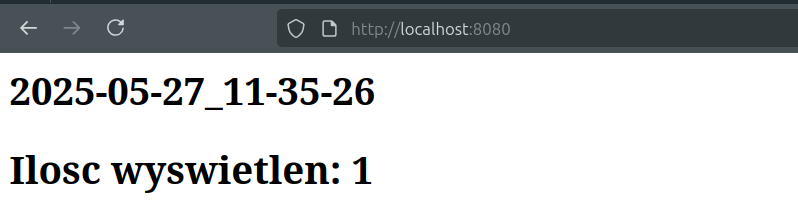
\includegraphics[width=\textwidth]{images/wysw_1.png}
            \caption{W przeglądarce połączono się z localhostem.}
            \label{fig:run_succes_2}
        \end{figure}

        \begin{figure}[ht]
            \centering
            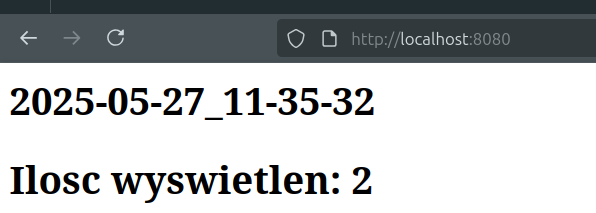
\includegraphics[width=\textwidth]{images/wysw_2.png}
            \caption{Po wyświetleniu Rys 1. Odświeżono przeglądarkę. Zwiększyła się liczba wyświetleń, godzina uległą zminaie.}
            \label{fig:run_succes}
        \end{figure}
\end{document}